
%!TEX root = ../main.tex

\section{Superconductivity of Nb}

With the help of an X-Y plotter, the resistance of niobium is determined as a function of the external magnetic field. The critical temperature is evaluated at the point where the resistance of niobium falls to half of the maximum value. It follows for the different magnetic field strengths:
\begin{table}
    \centering
    \caption{Critical temperature measurement values at critical magnetic field}
    \begin{tabular}{c|c|c}
        $ T_c$ in K&$I$ in A&$B_{c2}$ in T  \\
         \hline
         9,2& 0&0\\
         8,99&1,5&0,071895 \\
         8,84&3&0,14379 \\
         8,74&4,5&0,215685\\
         8,56&6&0,28758 \\
         8,45&7,5&0,359475 \\
         8,35&9&0,43137 \\
         8,25&10,5&0,503265 \\
    \end{tabular}
    \label{tab:Niob_critical}
\end{table}

The relationship between current and magnetic field was taken from the preparation folder
\footnote{Elektrische Leitfähigkeit von Festkörpern bei tiefen Temperaturen im Fortgeschrittenenpraktikum des Physikstudiums von Matthias Klaus Sickmüller, Page 34}
and the temperature was determined analogously to previous tasks with the carbon thermometer. 
\begin{figure}
    \centering
    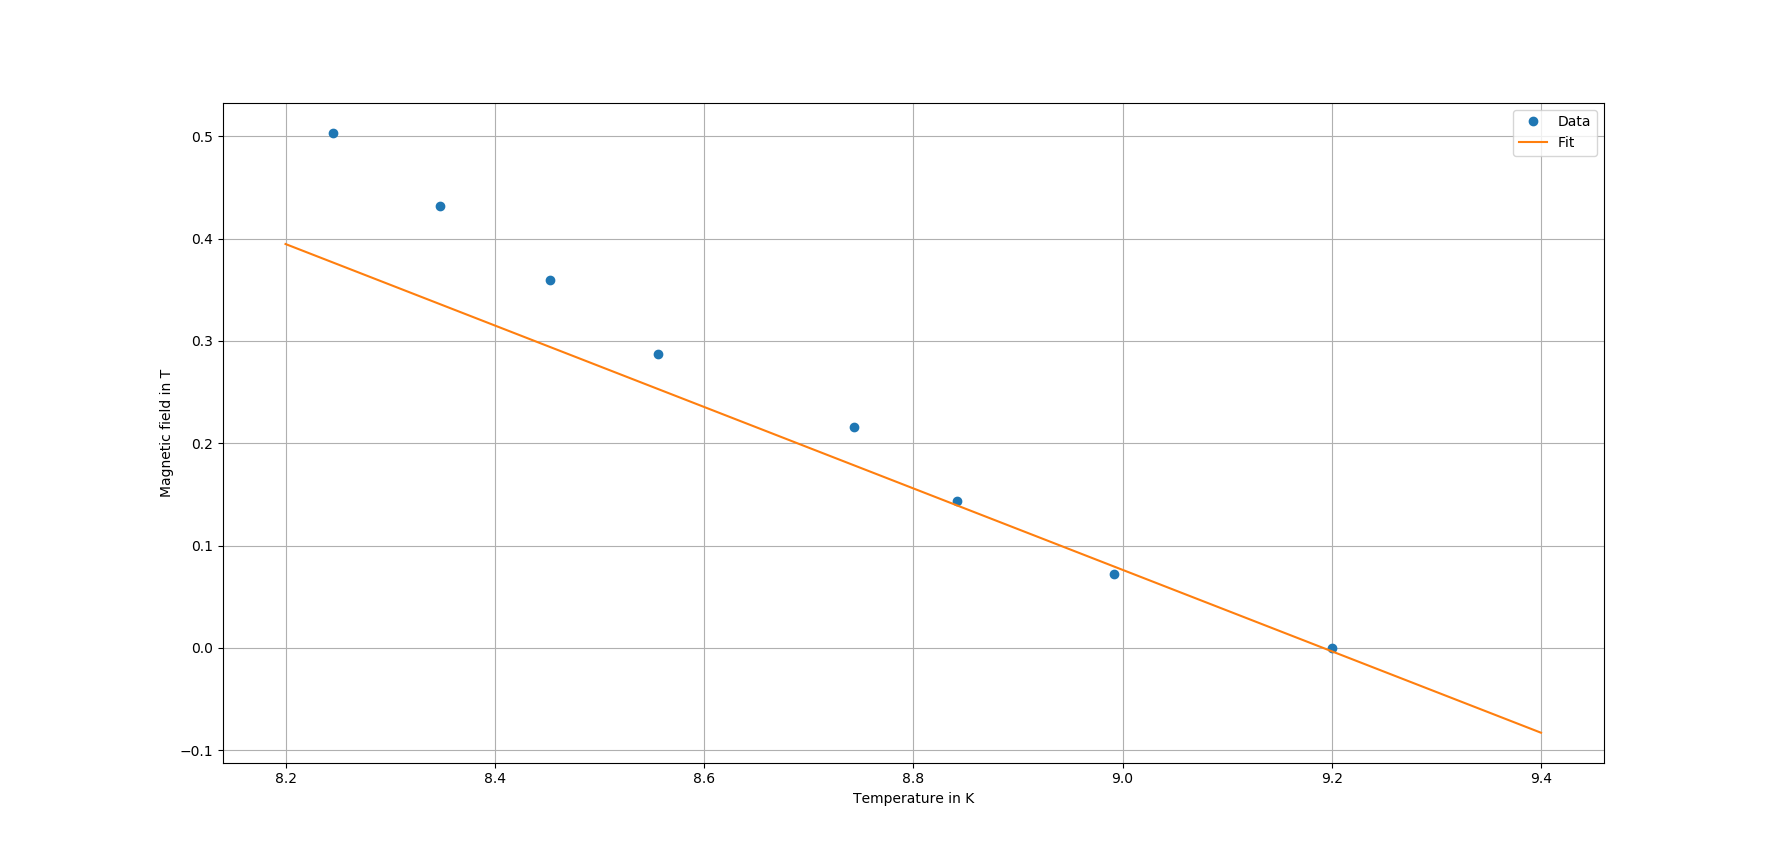
\includegraphics[width=1.0\textwidth]{./fig/ex3.png}
    \caption{Temperature dependency of upper critical field}
    \label{fig:Nb_B_T}
\end{figure}

In figure $\autoref{fig:Nb_B_T}$ it shows, as expected, that the critical temperature decreases with increasing magnetic field. Using a linear fit, the coherence length $\xi_{GL}(0)$ can now be determined to:
\begin{equation}
    \xi_{GL}(0)= \left[ \frac{-\Phi_0}{2\pi T_cA} \right]
\end{equation}
where $A$ corresponds to the gradient of the straight $f(x) = Ax+b$.  Thus, the coherence length is calculated as $\Phi_0 = \SI{2.07e-15}{Vs} $ to:

\begin{align*}
    A = \SI{-397,9\pm37,8 }{\frac{mT}{K}} \\
    \Rightarrow \xi_{GL}(0)= \SI{9,49\pm0,45}{nm} \\
\end{align*}
From the coherence length, the mean free path l for niobium can now be obtained via:
\begin{equation}
    l = \SI{2,31\pm0,22}{nm}
\end{equation}